%%%%%%%%%%%%%%%%%%%%%%%%%%%%%%%%%%%%%%%%%%%%%%%%%%%%
%%%             Metadata                         %%%
%%%%%%%%%%%%%%%%%%%%%%%%%%%%%%%%%%%%%%%%%%%%%%%%%%%%      

\title{Grundkurs Linguistik}

\subtitle{Sprache \& Sprachwissenschaft I}

\author[aMyP]{
	{\small Antonio Machicao y Priemer}
%	\\
%	{\footnotesize \url{http://www.linguistik.hu-berlin.de/staff/amyp}\\
%	\href{mailto:mapriema@hu-berlin.de}{mapriema@hu-berlin.de}}
}

\institute{Institut für deutsche Sprache und Linguistik}

%%%%%%%%%%%%%%%%%%%%%%%%%      
\date{ }
%\publishers{\textbf{6. linguistischer Methodenworkshop \\ Humboldt-Universität zu Berlin}}

%\hyphenation{nobreak}


%%%%%%%%%%%%%%%%%%%%%%%%%%%%%%%%%%%%%%%%%%%%%%%%%%%%
%%%             Preamble's End                   %%%
%%%%%%%%%%%%%%%%%%%%%%%%%%%%%%%%%%%%%%%%%%%%%%%%%%%%      


%%%%%%%%%%%%%%%%%%%%%%%%%      
\huberlintitlepage

\iftoggle{toc}{
\frame{
\begin{multicols}{2}
	\frametitle{Inhaltsverzeichnis}\tableofcontents
	%[pausesections]
\end{multicols}
	}
	}
%%%%%%%%%%%%%%%%%%%%%%%%%%%%%%%%%%%%%%%%%%%%%%%%%%%%%%%%%%
%%%%%%%%%%%%%%%%%%%%%%%%%%%%%%%%%%%%%%%%%%%%%%%%%%%%%%%%%
	
\section{Ziel des Kurses}

\iftoggle{toc}{
\frame{
\begin{multicols}{2}
	\tableofcontents[currentsection]
\end{multicols}
}
}
%%%%%%%%%%%%%%%%%%%%%%%%%%%%%%%%%%%%%%%%%%%%%%%%%%%%%%%%%%%%%

\begin{frame}{Ziel des Kurses}
		In diesem Kurs werden wir den folgenden Fragen nachgehen:
		
\begin{itemize}
		\item<1-> Was ist \textbf{Sprache}?
		\item<2-> Was ist \textbf{Sprachwissenschaft}?
		\item<3-> Welche \textbf{Ebenen} der Sprache sind bei ihrer Analyse zu berücksichtigen?
		\item<4-> Was sind die \textbf{Minimaleinheiten} der verschiedenen sprachlichen Ebenen und wie können diese miteinander \textbf{kombiniert} werden?
		\item<5-> Wie sehen linguistische \textbf{Fragestellungen} aus?
		\item<6-> Mit welchen \textbf{Methoden} können wir uns den Fragestellungen nähern?
		\item<7-> Außerdem: einige \textbf{Grammatiktheorien} (v.~a. in der Phonologie, Morphologie und Syntax) und einige linguistische Phänomene
\end{itemize}

\end{frame}


%%%%%%%%%%%%%%%%%%%%%%%%%%%%%%%%%%%%%%%%%%%%%%%%%%%%%%%%%%%%%%%%%%%%%%%%%%%%%%%%%%%%%%%%%%%%%%%%%%%%%%%%%%%%%%%%%%%%%%%%%%%%%%%%

\section{Sprache und natürliche Sprache}
\iftoggle{toc}{
\frame{
\begin{multicols}{2}
	\tableofcontents[currentsection]
\end{multicols}
}
}
%%%%%%%%%%%%%%%%%%%%%%%%%%%%%%%%%%%%%%%%%%%%%%%%%%%%%%%%%%%%%%%%

\begin{frame}{Sprache und natürliche Sprache}
	
\begin{itemize}
	\item Welches ist das \textbf{Untersuchungsgegenstand} der Linguistik? D.~h.: Was wird sprachwissenschaftlich untersucht und was nicht?
	\item[]
	\item Die Linguistik ist das Studium der \textbf{Sprache}, genauer der \textbf{natürlichen Sprachen}.
	\item[]
	\item Komplexe Definition von Sprache (wie die meisten Definitionen!)
	\item[]
	\item Terminus \gqq{Sprache} wird sehr vielfältig gebraucht.
\end{itemize}

\end{frame}

\begin{frame}

\begin{itemize}
	\item<1-> Duden Universalwörterbuch $\rightarrow$ weite Definition (vgl. \citet{Duden13a}):
	
	\begin{enumerate}
		\item<2->\label{DefSprache1} Die Sprache als \textbf{Fähigkeit} des Menschen zu sprechen.
		\item[]
		\item<3->\label{DefSprache2} Die Sprache im Sinne von \gqq{Sprechen} oder im Sinne von \gqq{\textbf{Rede}}.
		\item[]
		\item<4->\label{DefSprache3} Die Sprache als Redeweise oder als \textbf{Ausdrucksweise}.
		\item[]
		\item<5->\label{DefSprache4} Die Sprache als \textbf{System} von Zeichen und Regeln

		\begin{enumerate}
			\item[]
			\item<5->\label{DefSprache4a} als Verständigungsmittel für eine \textbf{Sprachgemeinschaft} oder
			\item[]
			\item<5->\label{DefSprache4b} als Kommunikationsmittel im \textbf{Allgemeinen}
		\end{enumerate}
			
	\end{enumerate}
	
\end{itemize}

\end{frame}


%%%%%%%%%%%%%%%%%%%%%%%%%%%%%%%%%%%%%%%%%%%%%%%%%%%%%%%%%%%%%

\begin{frame}
		
\begin{itemize}
	\item<1-> Weit gefasste Definition von Sprache $\rightarrow$ alle vier Punkte (von einem Universalwörterbuch zu erwarten!).
	\item[]
	\item<2-> ABER!: nicht \textit{nur} die menschliche Sprache, sondern auch \textbf{andere Arten von Kommunikationsmitteln} wie Tiersprachen, Körpersprache, künstliche Sprachen, etc. (s. Definition \ref{DefSprache4}) und ebenso \textbf{übertragene Bedeutungen} wie Sprache als Stil (s. Definition 	\ref{DefSprache3}), Sprache als \textbf{Handlung} (s. Definition \ref{DefSprache2}) oder Sprache als \textbf{Fähigkeit} (s. Definition \ref{DefSprache1}).
%	\item[]
%	\item<3-> Eng gefasste Definition von Sprache (als Gegenstand der Linguistik) \ras nur ein kleiner Teil der \textbf{Definitionen 1} (Sprache als Fähigkeit) und \textbf{4.1} (Sprache als Kommunikationsmittel einer Sprachgemeinschaft) 
%%Kommt auf nächster Folie noch mal! %%
\end{itemize}
		
\end{frame}


%%%%%%%%%%%%%%%%%%%%%%%%%%%%%%%%%%%%%%%%%%%%%%%%%%%%%%%%%%%%%

\begin{frame}

\begin{itemize}
	\item<1-> Eng gefasste Definition von Sprache (als Gegenstand der Linguistik) \ras nur ein kleiner Teil der \textbf{Definitionen 1} (Sprache als Fähigkeit) und \textbf{4.1} (Sprache als Kommunikationsmittel einer Sprachgemeinschaft)
	\item[]
	\item<2-> Auszug aus der Definition von \gqq{Sprache} aus dem \textit{Metzler Lexikon Sprache}:
\end{itemize}
			
\begin{block}<3->{Sprache}
    	   Wichtigstes und artspezif. Kommunikationsmittel der Menschen, das dem Austausch von Informationen dient sowie epistem. (die Organisation des Denkens betreffende), kognitive und affektive Funktionen erfüllt {[}\dots]. \citep{Glueck00a}
\end{block}
	
\end{frame}

%%%%%%%%%%%%%%%%%%%%%%%%%%%%%%%%%%%%%%%%%%%%%%%%%%%%%%%%%%%%%%

\begin{frame}

\begin{itemize}
	\item<1-> Demnach: Sprache (in erster Linie) \textbf{Kommunikationsmittel} zum Austausch von Informationen
	\item[]
	\item<2-> Sie ist \textbf{artspezifisch} ist, d.~h. dass nur Menschen eine Sprache (in dem oben genannten Sinne) haben\footnote{Vergleiche auch \citet{Bussmann83a}: \gqq{Sprache als eine {[}\dots] nur dem Menschen eigene Ausdrucksform {[}\dots]}.}.\\
	Siehe \textbf{Nim Chimpsky}:\\
	\url{http://www.npr.org/2011/07/20/138467156/project-nim-a-chimps-very-human-very-sad-life}
	\item[]
	\item<3-> Unterschied zwischen menschlicher Sprache, d.~h. der sog. \textbf{natürlichen Sprache}, und anderer Sprachformen wie Tiersprachen und Plansprachen (z.~B. Esperanto), formalen Sprachen (z.~B. C++), etc. (vgl. \citet{Thuemmel00a}).\
\end{itemize}		

\end{frame}


%%%%%%%%%%%%%%%%%%%%%%%%%%%%%%%%%%%%%%%%%%%%%%%%%%%%%%%%%%%%%%
%%%%%%%%%%%%%%%%%%%%%%%%%%%%%%%%%%%%%%%%%%%%%%%%%%%%%%%%%%%%%%%%
%
\subsection{Zeichensysteme}
%\frame{
%\begin{multicols}{2}
%\frametitle{~}
%	\tableofcontents[currentsection]
%\end{multicols}
%}
%%%%%%%%%%%%%%%%%%%%%%%%%%%%%%%%%%%%%%%%%%%%%%%%%%%%%%%%%%%%%%%%
	
\begin{frame}{Zeichensysteme}
			
\begin{itemize}
	\item<1-> Sprachen sind \textbf{Zeichensysteme}.
	\item<1-> Andere Zeichensysteme $\rightarrow$ Verkehrszeichen oder Partituren
	\item<2-> Zeichensysteme = Zeichen + Regeln zur Kombinatorik
	\item<3-> Zeichen = Formseite + Bedeutungs-/Funktionsseite
	\item<3-> Die Formseite ist abstrakt und kann graphisch, lautlich oder gestisch (im Falle von Gebärdensprachen) sein.
\end{itemize}			
			
%\begin{figure}[H]
%\centering
				
%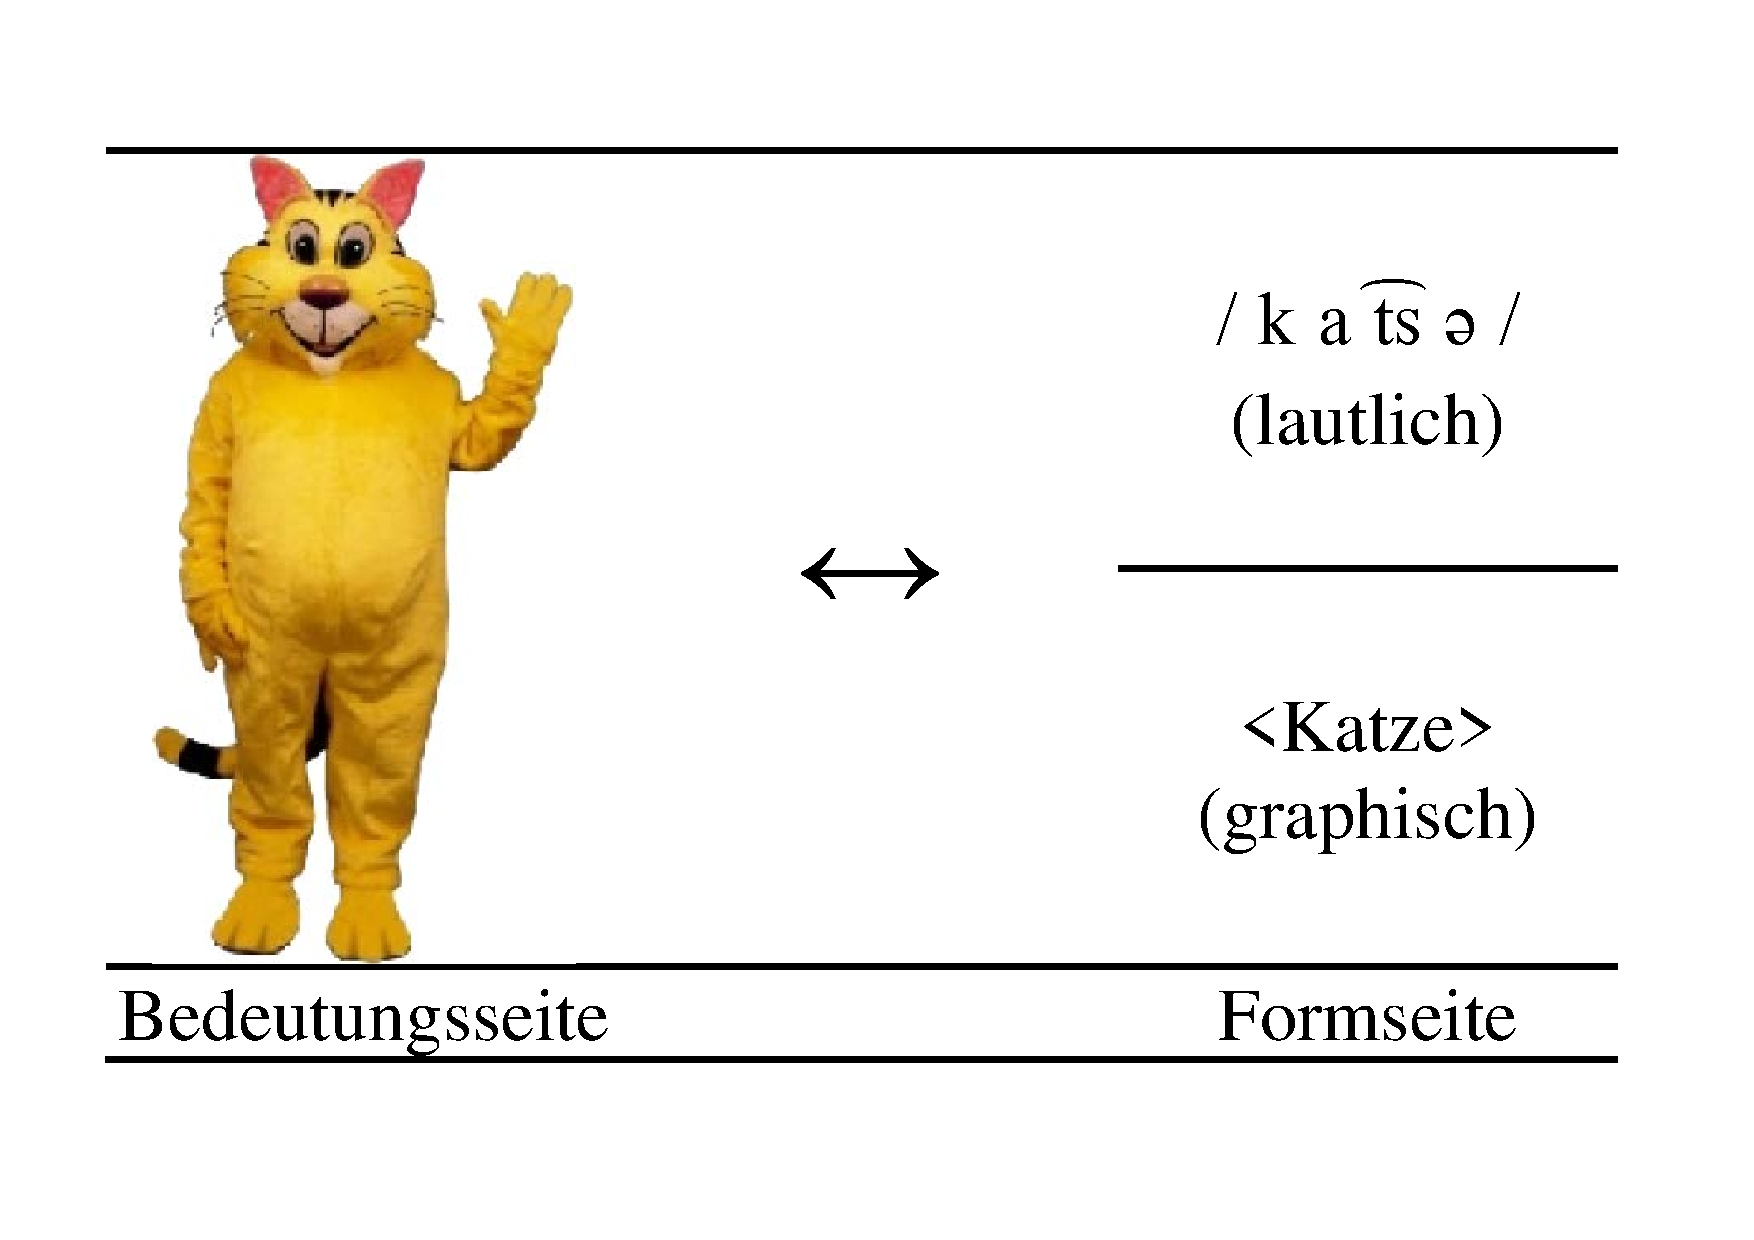
\includegraphics[scale=0.15]{material/01SSZeichenKatze}
%\caption{Beziehung zwischen Funktions-/Bedeutungs- und Formseite}
%\label{Zeichen1}
%\end{figure}

\end{frame}			

%%%%%%%%%%%%%%%%%%%%%%%%%%%%%%%%%%%%%%%%%%%%%%%%%%%%%%%%%%%%%%%%%%%%%%%%%%%%%%%%%%%%%%%%%%%%%%%%%%%%%%%%%%%%%%%%%

%Alternative zur Gelben Katze:

\begin{frame}
\begin{table}
\huge
\centering
%\caption[Hauskatze]{https://commons.wikimedia.org/wiki/File:Hauskatze_an_einem_Scheunenfenster_in_Grossarl.JPG; Autor: Usien; GNU Free Documentation Licence}
\begin{tabular}{lp{1em}l}
\hline
\multirow{4}*{
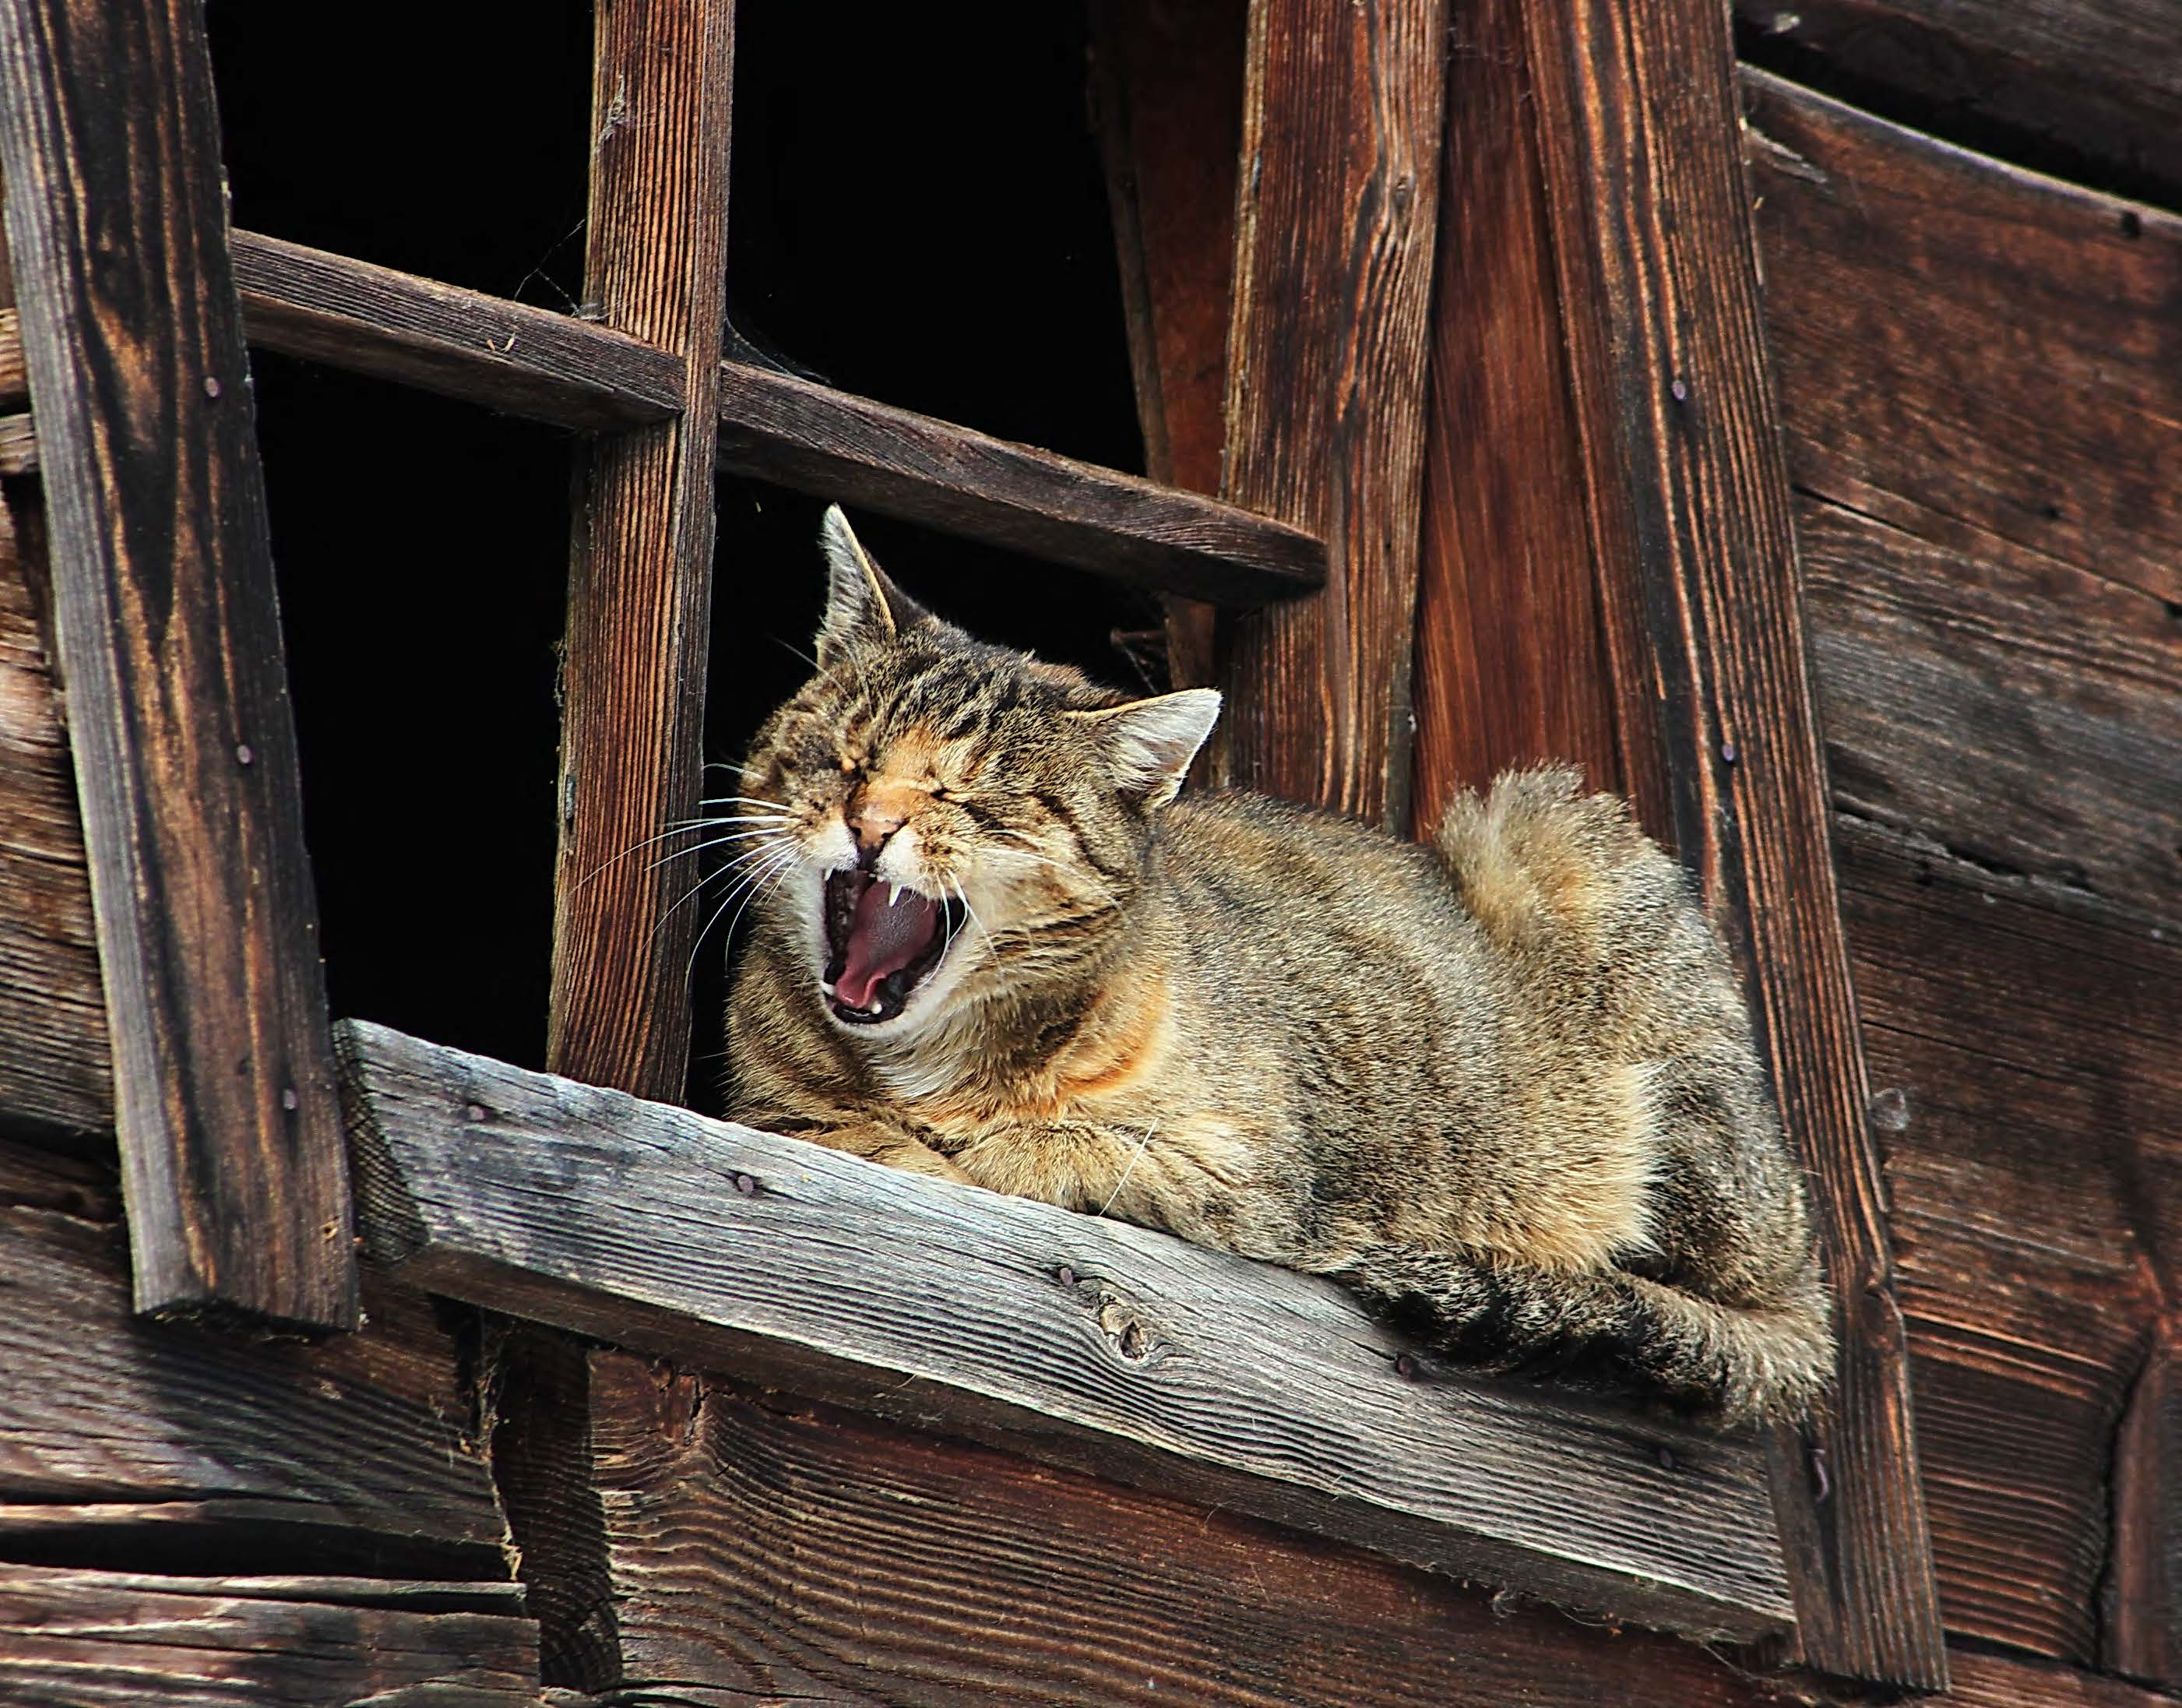
\includegraphics[scale=0.04]{material/Hauskatze-an-einem-Scheunenfenster-in-Grossarl}
}&  
%fehlt noch im Material-Ordner
\multirow{4}{6em}{{\LARGE $ \leftrightarrow $}} & / \textipa{k a \t{ts} \textschwa} / \\
& &(lautlich)\\
\cline{3-3}
& & $\langle$Katze$\rangle$\\
& &(graphisch)\\
\hline
Bedeutungsseite & & Formseite\\
\hline \\
\end{tabular}
\end{table}
\end{frame}


%%%%%%%%%%%%%%%%%%%%%%%%%%%%%%%%%%%%%%%%%%%%%%%%%%%%%%%%%%%%%%%%

\begin{frame}

\begin{itemize}
	\item<1-> \textbf{Tiere} verwenden auch Zeichensysteme zur Kommunikation.
\end{itemize}			
			
%\begin{figure}[H]
%\centering

%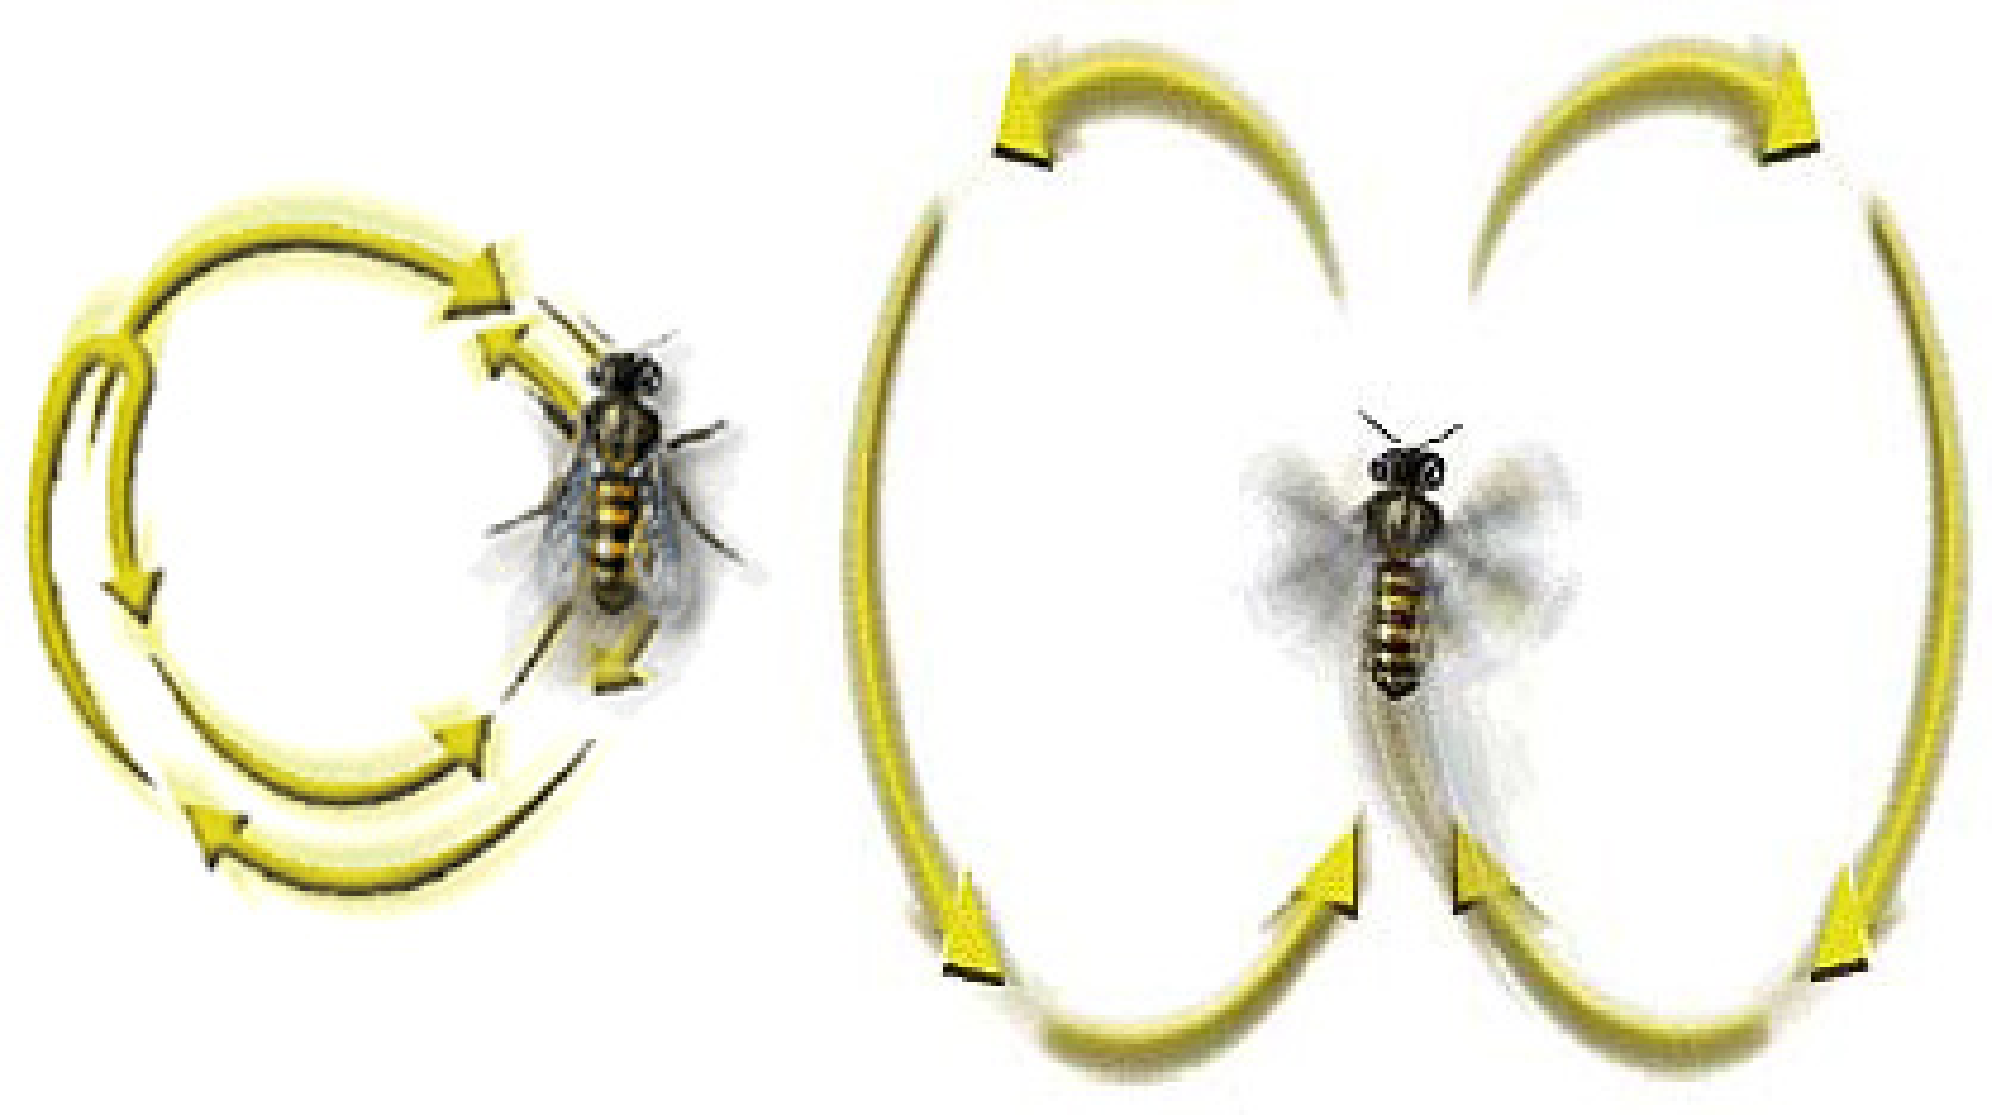
\includegraphics[scale=0.15]{material/01SSBienentanz}
%\caption{\gqq{Rundtanz} und \gqq{Schwänzeltanz} der Bienen}
%\label{Zeichen2}
%\end{figure}


\begin{figure}[H]
\centering

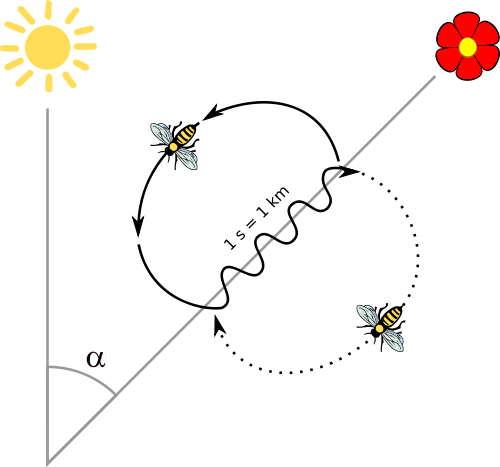
\includegraphics[scale=0.15]{material/Bee-dance}
\caption{https://commons.wikimedia.org/wiki/File:Bee\_dance.png?uselang=de; GNU-Lizenz; Autor:Audriusa; Bee\_dance/ Schwänzeltanz}
\label{Zeichen2}
\end{figure}

\begin{itemize}
	\item<2-> Mit diesem Zeichensystem teilen Bienen die \textbf{Richtung} und \textbf{Entfernung} der nächsten Nahrungsquelle mit. 
	\item<2-> Rundtanz: Trachtgebiet in der Nähe (weniger als 25m)
	\item<2-> Schwänzeltanz: Trachtgebiet bis zu 10km weit entfernt, weitere Bewegungen zeigen die Richtung an.
\end{itemize}		
		
\end{frame}			

\begin{frame}
\frametitle{Schwänzeltanz}

Imhoof, Markus. 2012: \emph{More than honey}, 13min 50sec



\end{frame}


%%%%%%%%%%%%%%%%%%%%%%%%%%%%%%%%%%%%%%%%%%%%%%%%%%%%%%%%%%%
%%%%%%%%%%%%%%%%%%%%%%%%%%%%%%%%%%%%%%%%%%%%%%%%%%%%%%%%%%%%
%
\subsection{Merkmale natürlicher Sprachen}
%\frame{
%\begin{multicols}{2}
%\frametitle{~}
%	\tableofcontents[currentsection]
%\end{multicols}
%}
%%%%%%%%%%%%%%%%%%%%%%%%%%%%%%%%%%%%%%%%%%%%%%%%%%%%%%%%%%
	
\begin{frame}{Merkmale natürlicher Sprachen}

\begin{itemize}
	\item Die menschliche (natürliche) Sprache unterscheidet sich jedoch von anderen Zeichensystemen, wie der \gqq{Bienensprache} oder den Verkehrszeichen, \textbf{nicht in einem einzelnen Merkmal}, sondern \textbf{in einem Bündel von Merkmalen}, welche alle zusammen vorhanden sein müssen (vgl. \citet{Hockett60a}).
\end{itemize}

\end{frame}


%%%%%%%%%%%%%%%%%%%%%%%%%%%%%%%%%%%%%%%%%%%%%%%%%%%%%%%%%%%%%


\begin{frame}

\begin{itemize}
	\item<1-> \textbf{Bidirektionalität:}

	\begin{itemize}
		\item[]
		\item<1-> Mensch ist \textbf{sowohl Sender als auch Empfänger} eines Sprachsignals.
		\item[]
		\item<2-> Bei einigen Singvögeln ist das anders:
		
		\begin{itemize}
			\item[]
			\item[$\rightarrow$]<2-> Während die Männchen singen, um ihr Revier zu markieren oder ein Weibchen anzulocken, können die Weibchen oft nicht oder nur wenig singen. Sie verstehen den Gesang der Männchen, können ihn aber selbst nicht produzieren.
		\end{itemize}
			
	\end{itemize}

\end{itemize}

\end{frame}


%%%%%%%%%%%%%%%%%%%%%%%%%%%%%%%%%%%%%%%%%%%%%%%%%%%%%%%%%%%%%

\begin{frame}

\begin{itemize}
	\item<1-> \textbf{Situationelle Ungebundenheit:}
	
	\begin{itemize}
		\item[]
		\item<1-> Menschen sind in der Lage auch über Dinge zu kommunizieren, die \textbf{nicht hier und jetzt} stattfinden.
		
		\begin{itemize}
			\item[]
			\item[$\rightarrow$]<2-> Wir können über das leckere gestrige Essen in der Mensa und über unsere Freude auf das morgige Mensafestmahl reden.
		\end{itemize}
		
		\item[]
		\item<3-> Der Tanz der Bienen ist in diesem Fall der menschlichen Kommunikation ähnlich.
		\item[]
		\item<3-> Einige Primaten sind jedoch nur in der Lage über das Hier und Jetzt zu kommunizieren.
	\end{itemize}
		
\end{itemize}

\end{frame}


%%%%%%%%%%%%%%%%%%%%%%%%%%%%%%%%%%%%%%%%%%%%%%%%%%%%%%%%%%%%%%%

\begin{frame}
	
\begin{itemize}
	\item<1-> \textbf{Rückkopplung:}
	
	\begin{itemize}
		\item<1-> Menschen können ihre \textbf{eigenen Sprachsignale} wahrnehmen und darauf reagieren.
		
\ea Ich habe heute \dots ääähhhh GESTERN die Hausaufgaben abgegeben.
\z

		\item<2->[$\rightarrow$] Der dreistachlige Stichling kann z.\,B. nicht die Färbung seiner Augen und seines Bauches wahrnehmen, die im Balzverhalten eine große Rolle spielt.
			\item[]
		\end{itemize}
			
	\item<3-> \textbf{Diskretheit:}
			
	\begin{itemize}
		\item<3-> Zeichen in natürlichen Sprachen können in kleine, diskrete (\textbf{von einander unterscheidbare}) \textbf{Einheiten} zerlegt werden.
				
		\begin{itemize}
			\item[]
			\item<4->[$\rightarrow$] Die Wörter\ab{Alben} und \ab{Alpen} unterscheiden sich nur in der Aussprache eines einzelnen Lautes.\\
					Vgl. \textipa{[\textglotstop{}alb@n]} vs. \textipa{[\textglotstop{}alp@n]}
			\item[]
			\item<4->[$\rightarrow$] Der Bienentanz ist eher kontinuierlich als diskret.						
		\end{itemize}
	
	\end{itemize}

\end{itemize}

\end{frame}


%%%%%%%%%%%%%%%%%%%%%%%%%%%%%%%%%%%%%%%%%%%%%%%%%%%%%%%%%%%%

\begin{frame}

\begin{itemize}
	\item<1-> \textbf{Produktivität:}
	
	\begin{itemize}
		\item[]				
		\item<1-> Eins der wichtigsten Merkmale natürlicher Sprachen!
		\item[]
		\item<2-> Aus einer \textbf{begrenzten Menge} von \textbf{Lauten} wird eine \textbf{(halb)begrenzte Menge} von \textbf{Wörtern} und daraus eine \textbf{unbegrenzte Menge} von \textbf{Sätzen} produziert ($\rightarrow$ offenes oder produktives System).
		\item[]
		\item<2-> Menschen können noch nie gehörte Sätze verstehen und noch nie gesagte Sätze produzieren.


\pause

\ea Meine Freundin hat gestern einen Wasserkocher mit Treueherzen von Kaiser's gekauft.
\ex Meine Freundin von Kaiser's hat gestern Treueherzen mit einem Wasserkocher gekauft.
\z
				
	\item<4-> Der Gibbon (kleiner Menschenaffe) hat ein geschlossenes Rufsystem mit einem kleinen \textbf{endlichen Inventar} an bekannten Lauten. 
	
	\end{itemize}
	
\end{itemize}

\end{frame}


%%%%%%%%%%%%%%%%%%%%%%%%%%%%%%%%%%%%%%%%%%%%%%%%%%%%%%%%%%%%%%%%

\begin{frame}

\begin{itemize}
	\item<1-> \textbf{Arbitrarität:}

	\begin{itemize}
		\item[]
		\item<1-> \textbf{Bezeichnendes} (Signifikant, frz. signifiant) ist nicht durch \textbf{Bezeichnetes} (Signifikat, frz. signifié) bestimmt!
		\item[]
		\item<2-> Verschiedene Sprachen haben unterschiedliche Namen (Bezeichendes) für das gleiche Objekt (Bezeichnetes):

\pause

\ea dt. \ab{Stift}, engl. \ab{pen}, sp. \ab{bolígrafo}, frz. \ab{crayon}, \dots
\z

		\item<4-> Benennung ist \textbf{konventionell}, d.\,h. in der Sprachgemeinschaft festgelegt.

		\begin{itemize}
			\item<5->[$\rightarrow$] Der Tanz der Bienen ist nicht arbiträr sondern motiviert!
		\end{itemize}
			
		\item[]
		\item<6-> Es gibt in natürlichen Sprachen \textbf{auch motivierte} Zeichen:
	
\ea Deutsch und Dänisch \textipa{[va\textupsilon{} va\textupsilon{}]}, Griechisch \textipa{[gav gav]}, Russisch \textipa{[gaf gaf]}, Spanisch \textipa{[g\textupsilon{}au g\textupsilon{}au]}, Französisch \textipa{[g\textupsilon{}af g\textupsilon{}af]}, Englisch \textipa{[w\textopeno{}f w\textopeno{}f]}, Litauisch \textipa{[a\textupsilon{} a\textupsilon{}]}, Koreanisch \textipa{[m\textopeno{}N m\textopeno{}N]}
\z
	
	\end{itemize}

\end{itemize}

\end{frame}


%%%%%%%%%%%%%%%%%%%%%%%%%%%%%%%%%%%%%%%%%%%%%%%%%%%%%%%%%%%%%%%%

\begin{frame}
		
	\begin{block}{Natürliche Sprache}
			Insgesamt bildet die natürliche Sprache also ein \textbf{produktives}, \textbf{bidirektionales}, \textbf{arbiträres} und \textbf{diskretes} Symbolsystem (vgl. \citet{Luedeling2009a}).
	\end{block}

\end{frame}	
